% This file is part of GUFI, which is part of MarFS, which is released
% under the BSD license.
%
%
% Copyright (c) 2017, Los Alamos National Security (LANS), LLC
% All rights reserved.
%
% Redistribution and use in source and binary forms, with or without modification,
% are permitted provided that the following conditions are met:
%
% 1. Redistributions of source code must retain the above copyright notice, this
% list of conditions and the following disclaimer.
%
% 2. Redistributions in binary form must reproduce the above copyright notice,
% this list of conditions and the following disclaimer in the documentation and/or
% other materials provided with the distribution.
%
% 3. Neither the name of the copyright holder nor the names of its contributors
% may be used to endorse or promote products derived from this software without
% specific prior written permission.
%
% THIS SOFTWARE IS PROVIDED BY THE COPYRIGHT HOLDERS AND CONTRIBUTORS "AS IS" AND
% ANY EXPRESS OR IMPLIED WARRANTIES, INCLUDING, BUT NOT LIMITED TO, THE IMPLIED
% WARRANTIES OF MERCHANTABILITY AND FITNESS FOR A PARTICULAR PURPOSE ARE DISCLAIMED.
% IN NO EVENT SHALL THE COPYRIGHT HOLDER OR CONTRIBUTORS BE LIABLE FOR ANY DIRECT,
% INDIRECT, INCIDENTAL, SPECIAL, EXEMPLARY, OR CONSEQUENTIAL DAMAGES (INCLUDING,
% BUT NOT LIMITED TO, PROCUREMENT OF SUBSTITUTE GOODS OR SERVICES; LOSS OF USE,
% DATA, OR PROFITS; OR BUSINESS INTERRUPTION) HOWEVER CAUSED AND ON ANY THEORY OF
% LIABILITY, WHETHER IN CONTRACT, STRICT LIABILITY, OR TORT (INCLUDING NEGLIGENCE
% OR OTHERWISE) ARISING IN ANY WAY OUT OF THE USE OF THIS SOFTWARE, EVEN IF
% ADVISED OF THE POSSIBILITY OF SUCH DAMAGE.
%
%
% From Los Alamos National Security, LLC:
% LA-CC-15-039
%
% Copyright (c) 2017, Los Alamos National Security, LLC All rights reserved.
% Copyright 2017. Los Alamos National Security, LLC. This software was produced
% under U.S. Government contract DE-AC52-06NA25396 for Los Alamos National
% Laboratory (LANL), which is operated by Los Alamos National Security, LLC for
% the U.S. Department of Energy. The U.S. Government has rights to use,
% reproduce, and distribute this software.  NEITHER THE GOVERNMENT NOR LOS
% ALAMOS NATIONAL SECURITY, LLC MAKES ANY WARRANTY, EXPRESS OR IMPLIED, OR
% ASSUMES ANY LIABILITY FOR THE USE OF THIS SOFTWARE.  If software is
% modified to produce derivative works, such modified software should be
% clearly marked, so as not to confuse it with the version available from
% LANL.
%
% THIS SOFTWARE IS PROVIDED BY LOS ALAMOS NATIONAL SECURITY, LLC AND CONTRIBUTORS
% "AS IS" AND ANY EXPRESS OR IMPLIED WARRANTIES, INCLUDING, BUT NOT LIMITED TO,
% THE IMPLIED WARRANTIES OF MERCHANTABILITY AND FITNESS FOR A PARTICULAR PURPOSE
% ARE DISCLAIMED. IN NO EVENT SHALL LOS ALAMOS NATIONAL SECURITY, LLC OR
% CONTRIBUTORS BE LIABLE FOR ANY DIRECT, INDIRECT, INCIDENTAL, SPECIAL,
% EXEMPLARY, OR CONSEQUENTIAL DAMAGES (INCLUDING, BUT NOT LIMITED TO, PROCUREMENT
% OF SUBSTITUTE GOODS OR SERVICES; LOSS OF USE, DATA, OR PROFITS; OR BUSINESS
% INTERRUPTION) HOWEVER CAUSED AND ON ANY THEORY OF LIABILITY, WHETHER IN
% CONTRACT, STRICT LIABILITY, OR TORT (INCLUDING NEGLIGENCE OR OTHERWISE) ARISING
% IN ANY WAY OUT OF THE USE OF THIS SOFTWARE, EVEN IF ADVISED OF THE POSSIBILITY
% OF SUCH DAMAGE.


\section{Database Schema}
\label{sec:schema}
GUFI stores extracted metadata in SQLite 3 database files. Each
directory contains a database file name db.db that contains a fixed
set of tables and views designed to facilitate efficient querying of
metadata.

\subsection{\entries}
The \entries table contains file and link metadata extracted from the
source filesystem using \stat, \readlink, and \listxattr. There are
also a few OS specific columns (\texttt{oss*}) that are currently
unused.

\subsection{Directory \summary}
The directory \summary table contains the metadata of the current
directory. Additionally, it contains columns that summarizes the
\entries table located in the same database file, such as minimum and
maximum file sizes, uids, and gids. These summary columns can be used
to determine whether or not \querydb needs to query the \entries table
at all.

\begin{figure} [h]
\centering
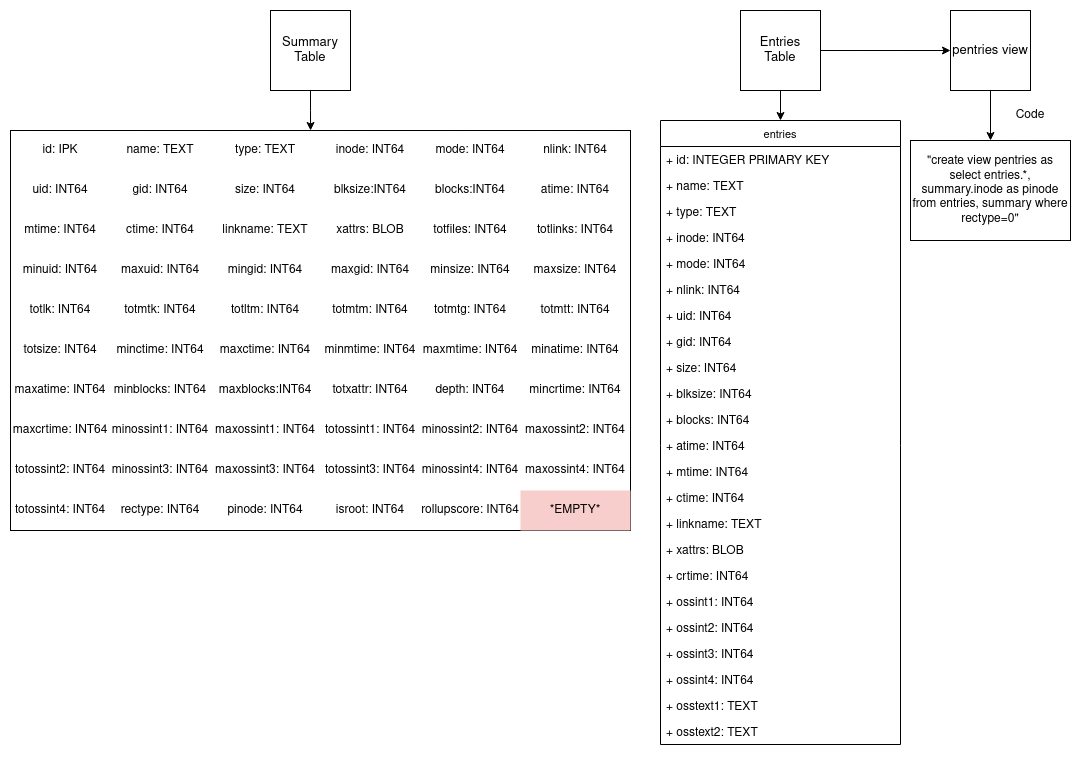
\includegraphics[width=1.0\textwidth]{images/Database_Schemas.png}
\caption{\label{fig:Database Schema}Database schema}
\end{figure}

\subsection{\pentries}
The original \pentries view was defined as:
\\\\
\texttt{SELECT entries.*, summary.inode FROM entries, summary};
\\\\
This was done in order to not store the parent inode of each entry,
which would be the same for every entry.

In general, users should query the \pentries view over the \entries
table in order to obtain complete sets of data to query on.

\subsubsection{\pentriesrollup}
In order to simplify rolling up indicies, the \pentries table was
modified to also union with the \pentriesrollup table, which contains
all child \pentries views copied into the current directory.

\subsection{\treesummary}
Similar to the directory \summary table, GUFI also provides
functionality to generate \treesummary tables. Instead of summarizing
only the data found in the entries table of the current directory, the
\treesummary table summarizes the contents of the entire subtree,
allowing for queries to completely skip processing entire subtries.

Generating \treesummary tables can be a very costly operation if done
on every single directory. Due to this, \treesummary tables are not
generated by default. Instead, they are generated by the \bfti
executable that must be run manually after indexing has completed.

\subsection{\vsummarydir}
The \vsummarydir view provides access to the entire directory summary
and not a partial directory summary (say by user or group).

\subsection{\vsummaryuser}
The \vsummaryuser view provides access to the directory summary for
each user (if this summary has been populated (not by default but
easily populatable via a query)).

\subsection{\vsummarygroup}
The \vsummarygroup view provides access to the directory summary for
each group (if this summary has been populated (not by default but
easily populatable via a query)).

\subsection{\vtsummarydir}
The vtsummarydir view provides access to the entire tree directory
summary and not a partial directory summary (say by user or group).

\subsection{\vtsummaryuser}
The \vtsummaryuser view provides access to the tree directory summary
for each user (if this summary has been populated (not by default but
easily populatable via a query)).

\subsection{\vtsummarygroup}
The \vtsummarygroup view provides access to the tree directory summary
for each group (if this summary has been populated (not by default but
easily populatable via a query)).

\subsection{\xattrs}
With the addition of extended attributes support, several more tables
and views were added into db.db. Additional database files with
different schemas were also added. See Section~\ref{sec:xattr_schema}
for details.
